\documentclass[manuscript,screen,nonacm]{acmart}

% LARA: Learned Adaptive Recombined Alignments.
% ACM single-column manuscript scaffold for an ICPM 2027 submission.

\usepackage{booktabs}
\usepackage{tikz}
\usetikzlibrary{positioning,fit,backgrounds,arrows.meta,calc}
\usepackage{pgfplots}
\pgfplotsset{compat=1.16}
\usepackage{algorithm}
\usepackage{algpseudocode}

% Entity-stable series colors used across all charts:
% LARA (guided fast mode) is always blue, the exact backend is always aqua.
\definecolor{seriesblue}{HTML}{2A78D6}
\definecolor{seriesaqua}{HTML}{1BAF7A}

\pgfplotsset{
  larachart/.style={
    width=0.54\linewidth,
    height=0.26\linewidth,
    axis lines=left,
    axis line style={black!45},
    tick style={black!45},
    grid=major,
    major grid style={line width=0.4pt, draw=black!12},
    ticklabel style={font=\footnotesize, color=black!70},
    label style={font=\footnotesize},
    legend style={draw=none, fill=none, font=\footnotesize, legend cell align=left},
    every axis plot/.append style={line width=1.1pt},
  },
  larapanel/.style={
    larachart,
    width=\linewidth,
    height=0.34\linewidth,
  }
}

% Shared styles for the two architecture diagrams. The learned (blue) and
% exact (aqua) stages reuse the entity-stable series colors of the charts.
\tikzset{
  larabox/.style={draw, rounded corners=2.5pt, align=center, inner xsep=5pt,
    inner ysep=4pt, minimum height=9.5mm, line width=0.7pt},
  learnedbox/.style={larabox, draw=seriesblue!75!black, fill=seriesblue!9},
  exactbox/.style={larabox, draw=seriesaqua!70!black, fill=seriesaqua!12},
  iobox/.style={larabox, draw=black!55, fill=black!4},
  stagebg/.style={rounded corners=5pt, inner sep=3mm},
  stagelab/.style={font=\scriptsize\itshape, inner sep=1.5pt},
  flow/.style={-{Stealth[length=2.4mm, width=2mm]}, line width=0.9pt, draw=black!60},
  biflow/.style={{Stealth[length=2.2mm, width=1.8mm]}-{Stealth[length=2.2mm, width=1.8mm]},
    line width=0.9pt, draw=black!60},
  flowlab/.style={font=\scriptsize, text=black!65, align=center, inner sep=1.5pt},
}
% Tiny icons drawn as pics in the host picture: a place-transition-place
% fragment and a three-event trace, both centered at the pic origin.
\tikzset{
  pics/pnfrag/.style={code={
    \draw[black!70, sharp corners] (-1.9mm,-1.4mm) rectangle (-0.7mm,1.4mm);
    \fill[black!25] (-1.9mm,-1.4mm) rectangle (-0.7mm,1.4mm);
    \draw[black!70] (-4.4mm,0) circle (1.3mm);
    \fill[black!70] (-4.4mm,0) circle (0.55mm);
    \draw[black!70] (3.1mm,0) circle (1.3mm);
    \draw[black!70, -{Stealth[length=1.1mm]}] (-3.0mm,0) -- (-2.0mm,0);
    \draw[black!70, -{Stealth[length=1.1mm]}] (-0.6mm,0) -- (1.7mm,0);}},
  pics/trcfrag/.style={code={
    \foreach \i/\l in {-1/a,0/b,1/c} {
      \draw[black!70, fill=black!8, sharp corners]
        (\i*3.3mm-1.35mm,-1.5mm) rectangle +(2.7mm,3mm);
      \node[font=\tiny, text=black!70, inner sep=0pt] at (\i*3.3mm,0) {$\l$};}}},
  pics/algfrag/.style={code={
    \foreach \i/\t/\b in {-1/$a$/$t_1$, 0/$b$/$\gg$, 1/$\gg$/$t_2$} {
      \draw[black!70, fill=black!8, sharp corners]
        (\i*3.3mm-1.35mm,0mm) rectangle +(2.7mm,2.8mm);
      \draw[black!70, fill=seriesblue!12, sharp corners]
        (\i*3.3mm-1.35mm,-2.8mm) rectangle +(2.7mm,2.8mm);
      \node[font=\tiny, text=black!70, inner sep=0pt] at (\i*3.3mm,1.4mm) {\t};
      \node[font=\tiny, text=black!70, inner sep=0pt] at (\i*3.3mm,-1.4mm) {\b};}}},
}

% Colors for the latent regions of the diagnostic decomposition branch
% (distinct from the entity-stable series colors of the charts).
\definecolor{regamber}{HTML}{D97E22}
\definecolor{regplum}{HTML}{8E5BC0}
\definecolor{regslate}{HTML}{5E7A8A}

% Styles for the worked-example figures: Petri net elements, score badges,
% and the two-row alignment table of the decoding example.
\tikzset{
  place/.style={circle, draw=black!70, minimum size=4.2mm, inner sep=0pt,
    line width=0.6pt},
  trans/.style={rectangle, draw=black!70, minimum width=4.8mm,
    minimum height=4.8mm, inner sep=1pt, line width=0.6pt, font=\small},
  invtrans/.style={trans, fill=black!75, text=white},
  netarc/.style={-{Stealth[length=1.6mm]}, black!70, line width=0.6pt},
  scorebadge/.style={draw=seriesblue!75!black, fill=seriesblue!12,
    rounded corners=1.5pt, inner sep=1.8pt, font=\scriptsize},
  scorebadgelow/.style={draw=black!45, fill=black!5, rounded corners=1.5pt,
    inner sep=1.8pt, font=\scriptsize, text=black!60},
  alcell/.style={rectangle, draw=black!60, minimum width=13mm,
    minimum height=5.2mm, inner sep=1pt, font=\small},
  regbox/.style={rounded corners=3pt, dashed, inner sep=2mm, line width=0.7pt},
  reglab/.style={font=\scriptsize\itshape, inner sep=1pt},
}

\acmConference[ICPM '27]{International Conference on Process Mining 2027}{TBD 2027}{TBD}
\acmYear{2027}
\copyrightyear{2027}
\acmDOI{TODO}
\acmISBN{TODO}

\title[LARA: Learned Adaptive Recombined Alignments]{LARA: Learned Adaptive Recombined Alignments, a Certifying Foundation Model for Petri Net Trace Alignment}

\author{Alessandro Berti}
\orcid{0000-0002-3279-4795}
\affiliation{%
  \institution{Process and Data Science (PADS), RWTH Aachen University}
  \city{Aachen}
  \country{Germany}}
\email{a.berti@pads.rwth-aachen.de}

\author{Wil M.P. van der Aalst}
\orcid{0000-0002-0955-6940}
\affiliation{%
  \institution{Process and Data Science (PADS), RWTH Aachen University}
  \city{Aachen}
  \country{Germany}}
\affiliation{%
  \institution{Celonis}
  \city{Munich}
  \country{Germany}}
\email{wvdaalst@pads.rwth-aachen.de}

\renewcommand{\shortauthors}{Alessandro Berti et al.}

\begin{abstract}
Alignments explain, event by event, how a trace deviates from a process model, but computing an optimal alignment requires exact shortest-path search, often the bottleneck on real discovered models. Purely learned aligners are fast but may return illegal or silently suboptimal alignments. LARA (Learned Adaptive Recombined Alignments) combines both: a small neural foundation model, trained once on synthetic data and applicable to any net and any log without retraining, scores alignment moves; a constrained decoder turns the scores into a candidate; exact replay verifies it; and an exact backend certifies or repairs it on demand. Every answer is therefore a legal alignment with a known cost, and optionally a certified optimal one. In the assessment, all produced alignments are legal and 91\% attain the exact optimal cost. An ablation attributes the learned contribution specifically to the resolution of duplicate labels. Legality transfers zero-shot to stress nets and real-life logs, and the fast path overtakes exact search on larger nets and on real discovered models dominated by invisible transitions.
\end{abstract}

\ccsdesc[500]{Information systems~Business process management}
\ccsdesc[300]{Computing methodologies~Modeling methodologies}

\keywords{process mining, conformance checking, alignments, Petri nets, neural networks, certification}

\begin{document}

\maketitle

\section{Introduction}
\label{sec:introduction}

Process mining relates recorded event data to process models in order to discover, check, and improve processes \cite{Aalst2016}. Conformance checking quantifies how well observed behavior agrees with modeled behavior \cite{Carmona2018,Rozinat2008}, and alignments are its reference technique \cite{Adriansyah2011,Adriansyah2014}: an alignment explains every event of a trace through synchronous, log, and model moves, and an optimal alignment minimizes the total deviation cost. The result is not merely a fitness number but a diagnostic object showing exactly where log and model disagree.

The guarantee of optimality is also the computational bottleneck of the technique. Optimal alignments are computed by exact shortest-path search, typically A* \cite{Hart1968} with heuristics derived from the marking equation \cite{Dongen2018,Zelst2018}, over the reachability graph of a synchronous product net. This state space grows with concurrency, loops, duplicate labels, and invisible transitions, and the problem is intrinsically hard \cite{Schwanen2026}. These constructs occur frequently in discovered models, so exact alignment can dominate the running time of a conformance analysis and can exhibit substantial variance across traces.

Neural models have been applied successfully to event data for predictive monitoring and discovery \cite{Tax2017,Bukhsh2021,Sommers2021}, and they offer a possible way to obtain low-latency alignment candidates. However, a purely learned aligner is not sufficient for conformance checking unless its output is checked against the process semantics: a predicted alignment may be \emph{illegal}, meaning that its model projection cannot be replayed from the initial to the final marking, or it may be suboptimal without an explicit certificate. A learned alignment method therefore has to address both computational efficiency and semantic correctness.

This paper studies such a hybrid design. We present LARA (Learned Adaptive Recombined Alignments), a neural-guided alignment system built around the invariant that \emph{neural output is never used as a certificate}. A learned model scores alignment decisions; a constrained greedy decoder turns the scores into a candidate whose model moves are fireable by construction; an exact replay verifier checks legality; and an exact alignment backend remains responsible for optimality, certifying or repairing the candidate. The neural component is used to propose candidates, while replay and exact search provide the guarantees. Figure~\ref{fig:outline} summarizes the learned core of the approach and the outputs it produces.

The design has three relevant properties. First, the neural component is a small \emph{foundation model} for alignment: it is trained once, offline, on synthetic data, and it uses hashed label embeddings rather than a fixed activity vocabulary, so the same checkpoint can be applied to different event logs and Petri nets without retraining. Second, its per-trace latency is largely determined by feature extraction and one forward pass, whereas exact search may have heavy-tailed running times on some traces. Third, every returned candidate is replay-verified and has a known cost; in certified mode, cost equality with the exact backend provides the same optimality guarantee as classical alignment. The contribution of the paper is this \textbf{foundation model for alignment}, one neural model that scores alignment moves for arbitrary Petri nets and event logs, together with the certifying architecture that separates proposal from verification (Section~\ref{sec:approach}), the exact-labeled synthetic pipeline used for training, and an assessment of the learned contribution, the speed threshold relative to exact A*, and zero-shot transfer to real-life logs (Section~\ref{sec:assessment}).

We evaluate the approach through six research questions. \textbf{RQ1 (legality)}: are the produced alignments always legal, even on unseen nets and vocabularies? \textbf{RQ2 (near-optimality)}: how often is the exact optimal cost attained, and how large are the gaps otherwise? \textbf{RQ3 (ambiguity)}: are duplicate labels and invisible routing resolved? \textbf{RQ4 (generalization)}: does performance transfer across families, scales, and real-life logs? \textbf{RQ5 (certification)}: how often does cost equality certify the candidate? \textbf{RQ6 (attribution)}: how much quality is owed to the learned scores rather than to the constrained search around them?

\begin{figure}
\centering
\resizebox{0.76\textwidth}{!}{%
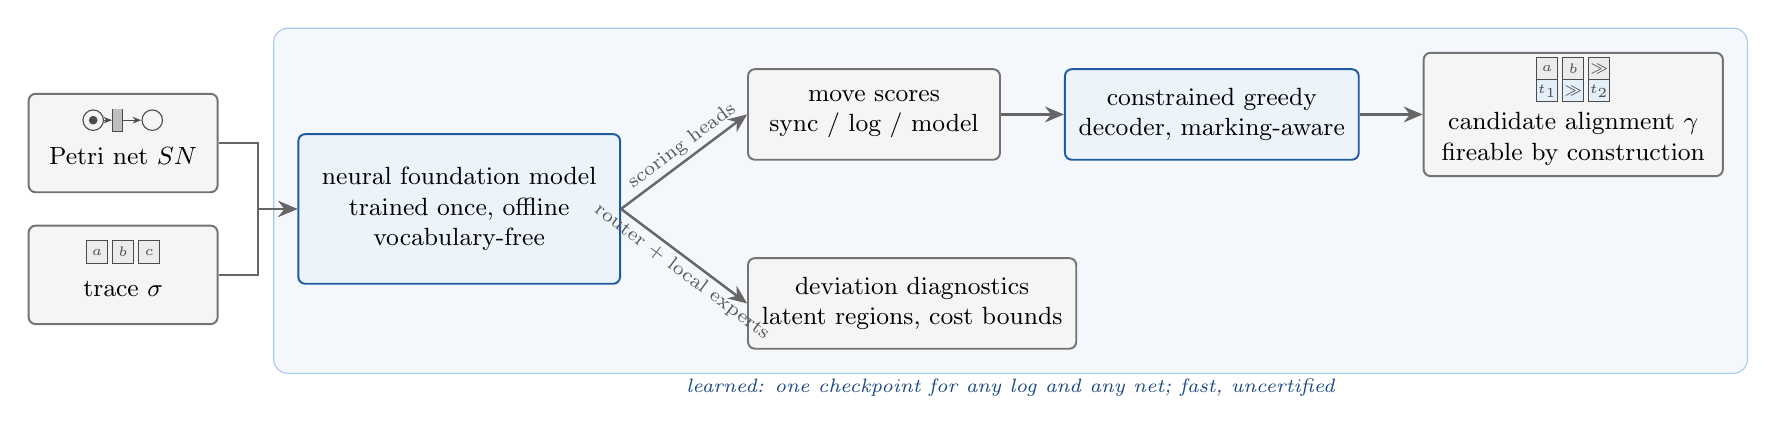
\begin{tikzpicture}[font=\small, node distance=4mm and 6mm]
% inputs
\node[iobox, minimum width=24mm, minimum height=12.5mm] (net) {~\\[1.5mm] Petri net $SN$};
\node[iobox, minimum width=24mm, minimum height=12.5mm, below=4mm of net] (trace) {~\\[1.5mm] trace $\sigma$};
\pic at ($(net.center)+(0.6mm,2.9mm)$) {pnfrag};
\pic at ($(trace.center)+(0,2.9mm)$) {trcfrag};
\coordinate (inmid) at ($(net.east)!0.5!(trace.east)$);
% the foundation model
\node[learnedbox, right=10mm of inmid, anchor=west, minimum height=19mm, inner xsep=3mm] (fm) {neural foundation model\\trained once, offline\\vocabulary-free};
% direct outputs: move scores (top) and diagnostics (bottom)
\node[iobox, right=16mm of fm.east, anchor=west, yshift=12mm, minimum width=32mm, minimum height=11.5mm] (scores) {move scores\\sync / log / model};
\node[iobox, right=16mm of fm.east, anchor=west, yshift=-12mm, minimum width=32mm, minimum height=11.5mm] (diag) {deviation diagnostics\\latent regions, cost bounds};
% the scores feed the decoder, which emits the candidate
\node[learnedbox, right=8mm of scores, minimum height=11.5mm] (dec) {constrained greedy\\decoder, marking-aware};
\node[iobox, right=8mm of dec, minimum width=38mm, minimum height=15.5mm] (cand) {~\\[4.5mm] candidate alignment $\gamma$\\fireable by construction};
\pic at ($(cand.center)+(0,4.4mm)$) {algfrag};
% flows
\draw[flow] (net.east) -- ++(5mm,0) |- (fm.west);
\draw[flow] (trace.east) -- ++(5mm,0) |- (fm.west);
\draw[flow] (fm.east) -- node[flowlab, above, sloped, pos=0.55] {scoring heads} (scores.west);
\draw[flow] (fm.east) -- node[flowlab, below, sloped, pos=0.55] {router $+$ local experts} (diag.west);
\draw[flow] (scores) -- (dec);
\draw[flow] (dec) -- (cand);
% stage background
\begin{scope}[on background layer]
\node[stagebg, fill=seriesblue!5, draw=seriesblue!40] (learnedbg) [fit=(fm)(scores)(dec)(cand)(diag)] {};
\end{scope}
\node[stagelab, text=seriesblue!60!black, anchor=north] at (learnedbg.south) {learned: one checkpoint for any log and any net; fast, uncertified};
\end{tikzpicture}}
\caption{The LARA foundation model for alignment: trained once, offline, and vocabulary-free, it maps any Petri net and trace pair to move scores and to deviation diagnostics; the move scores in turn drive a constrained, marking-aware greedy decoder whose candidate alignment is fireable by construction. All outputs are fast but uncertified.}
\label{fig:outline}
\end{figure}

Section~\ref{sec:relatedWork} positions LARA in the literature, Section~\ref{sec:preliminaries} fixes notation, Section~\ref{sec:approach} details the approach, Section~\ref{sec:assessment} reports the assessment, and Sections~\ref{sec:discussion} and~\ref{sec:conclusion} discuss and conclude.

\section{Related Work}
\label{sec:relatedWork}

\textbf{Foundations and alignments.} Petri nets \cite{Murata1989} remain central to conformance checking \cite{Aalst2016,Carmona2018}. Replay-based conformance checking links trace events to model elements \cite{Rozinat2008}; cost-based alignments \cite{Adriansyah2011,Adriansyah2014} introduced the synchronous, log, and model move vocabulary used throughout this paper, and van Zelst et al.\ \cite{Zelst2018} formalize alignment computation as a shortest-path problem over a synchronous product. LARA preserves this diagnostic tradition: its output is an alignment object with transition identities, not a predicted score.

\textbf{Exact search and acceleration.} Efficient exact methods refine A* \cite{Hart1968} with (extended) marking-equation heuristics \cite{Dongen2018} or reduce explored states as in REACH \cite{Casas2024}; complexity analyses underline why the problem resists such optimizations in general \cite{Schwanen2026}. These approaches provide formal guidance inside one search; LARA instead provides empirical guidance outside the exact search and keeps the exact layer for certification only.

\textbf{Decomposition and recomposition.} Decomposing nets speeds up conformance checking \cite{Aalst2013}, local alignments can be merged \cite{Verbeek2016}, recomposition restores exact results or bounds \cite{Lee2018}, and automata with S-components offer another scalable route \cite{Reissner2020}. LARA is architecturally close to this family, but its regions are latent and trace-dependent rather than fixed structural decompositions.

\textbf{Approximate conformance checking.} Token-based replay \cite{Rozinat2008,Berti2021}, alignment approximation for process trees \cite{Schuster2021}, and relaxation labeling \cite{Padro2022} occupy the same speed and accuracy space as LARA's fast mode. The distinctive feature of LARA is the certification boundary: candidates are replay-verified, then certified by cost equality or repaired exactly.
\textbf{Neural methods in process mining.} Neural models of event data have mostly targeted prediction, with recurrent networks \cite{Tax2017}, transformers \cite{Vaswani2017,Bukhsh2021}, and graph neural networks for discovery \cite{Sommers2021}; a recent survey identifies conformance checking as an open opportunity for AI \cite{Genga2025}. None of these works constructs legal, costed alignments against an explicit Petri net; LARA is a concrete instance of that agenda.

\textbf{Learning-augmented search.} Outside process mining, machine learning guides combinatorial optimization \cite{Bengio2021} and shortest-path search, as in Neural A* \cite{Yonetani2021}. LARA is deliberately more conservative: learned scores rank moves for a greedy decoder and are never used as admissible heuristics, so the trust model of exact conformance checking is preserved. The gap LARA addresses is thus \emph{certifiable neural guidance} for Petri net trace alignment.

\section{Preliminaries}
\label{sec:preliminaries}

\textbf{Events, traces, and logs.} Let $\mathcal{A}$ be a finite alphabet of activity labels. A trace $\sigma = \langle a_1, \ldots, a_n \rangle \in \mathcal{A}^*$ is a finite sequence of events describing one case; an event log is a multiset of traces. We align a single trace against a model; log-level results follow by aggregation.

\textbf{Labeled Petri nets.} A Petri net is a tuple $N = (P, T, F)$ with places $P$, transitions $T$, $P \cap T = \emptyset$, and flow relation $F \subseteq (P \times T) \cup (T \times P)$. A marking $m : P \to \mathbb{N}$ assigns tokens to places; a transition is enabled iff all its input places carry a token, and firing it consumes from input and produces into output places, written $m \xrightarrow{t} m'$. A labeling function $\lambda : T \to \mathcal{A} \cup \{\tau\}$ marks transitions as visible or invisible ($\tau$); invisible transitions represent routing that leaves no trace in the log, and two distinct transitions may share a visible label (duplicate labels). Both phenomena are central here: an observed event determines the \emph{label} of a matching transition but not its \emph{identity}. A system net $SN = (N, m_0, m_f)$ adds initial and final markings.

\textbf{Alignments.} Let $\gg$ denote a skip symbol. A move is a pair $(x, y) \in (\mathcal{A} \cup \{\gg\}) \times (T \cup \{\gg\})$, excluding $(\gg, \gg)$: a synchronous move $(a, t)$ with $\lambda(t) = a$, a log move $(a, \gg)$, or a model move $(\gg, t)$. An alignment of $\sigma$ and $SN$ is a sequence of moves $\gamma$ such that (1) the sequence of non-$\gg$ log components equals $\sigma$ exactly, and (2) the sequence of non-$\gg$ model components is a firing sequence of $N$ from $m_0$ that reaches $m_f$. An alignment satisfying both conditions is \emph{legal}. Moves carry the transition identity $t$, not just its label: with duplicate labels, two alignments can have identical label projections yet fire different transitions.

\textbf{Costs and optimality.} The standard unit cost model charges $0$ for synchronous moves and invisible model moves and $1$ for log moves and visible model moves. The cost of an alignment is $c(\gamma) = \sum_i c(x_i, y_i)$, and an alignment is optimal iff its cost equals $\delta(\sigma, SN) = \min \{ c(\gamma) \mid \gamma \text{ legal} \}$. Optimal alignments need not be unique; the optimal cost is, and under unit costs it counts the minimum number of deviations needed to explain the trace.

\textbf{Synchronous product and A*.} The classical construction builds a synchronous product of $SN$ and a linear trace net; legal alignments correspond exactly to complete firing sequences of the product, so computing an optimal alignment is a shortest-path problem over its reachability graph \cite{Zelst2018}, solved by A* with admissible heuristics from the (extended) marking equation \cite{Dongen2018}. We use the state-equation A* aligner of PM4Py \cite{Berti2023} as exact backend and as the source of ground-truth labels.

\textbf{Certification.} A certificate of optimality for a candidate $\gamma$ is a proof that $c(\gamma) = \delta(\sigma, SN)$. Two routes provide such a proof: the marking equation yields a lower bound on $\delta$ \cite{Dongen2018}, so a legal candidate whose cost meets this bound is optimal without any search, and the exact solver returns $\delta$ itself, so cost equality certifies a legal candidate even if it differs from the exact alignment. The paper uses cost equality as its certification rule.

\section{Approach}
\label{sec:approach}

LARA separates \emph{candidate generation} (learned, fast, uncertified) from \emph{certification} (exact, trusted). Figure~\ref{fig:architecture} shows the pipeline. At alignment time a net and trace pair passes through three stages, each consuming exactly what the previous one produces: input encoding re-encodes the pair for the neural model (Section~\ref{sec:encoding}), the neural model scores the possible moves (Section~\ref{sec:architecture}), and the decoder turns the scores into one alignment that exact methods then verify and certify (Section~\ref{sec:decoding}). Sections~\ref{sec:data} and~\ref{sec:training} describe the offline training of the neural model, which happens once and is amortized over all later use.


\subsection{Input Encoding: Reading the Net and the Trace}
\label{sec:encoding}

\emph{Input:} a system net $SN = (N, m_0, m_f)$ and a trace $\sigma$ of length $n$. \emph{Output:} a graph view of the net, the trace as a sequence of label identifiers, and a compatibility mask $C$ recording which event and transition pairs share a label.

\textbf{The net as a typed graph.} The net is encoded as a bipartite graph with one node per place and one node per transition. Encoding the net itself, rather than any behavioral expansion of it, keeps the input linear in the size of the net; the reachability graph, whose potentially exponential size is what makes exact alignment expensive, is never materialized. The node attributes are chosen so that every quantity the move scorer must weigh is locally visible. Place nodes carry their token counts in the initial and final markings and their degrees: the markings tell the model where execution starts and where it must end, and the degrees mark branching and synchronization points. Transition nodes carry their invisibility flag and their move costs, since inserting a $\tau$ is free while a visible model move is penalized, together with their degrees and a self-loop context flag, which signal local choice, concurrency, and repeatable behavior. Every arc contributes two edges, one per direction, with the direction recorded as the edge type. Keeping direction observable preserves the firing semantics: an undirected edge could not distinguish a preset place, which enables a transition, from a postset place, which receives its tokens. The reverse edges are added because the information that distinguishes two transitions sharing a label typically lies \emph{downstream} of them, for example in the branch suffix that follows each. If messages flowed only along arc direction, two duplicates with symmetric presets would receive provably identical representations; with edges in both directions, the disambiguating suffix reaches each duplicate in two hops (Section~\ref{sec:ablation}).

\textbf{Activity labels without a vocabulary.} Activity labels are mapped to a bounded set of 8{,}192 identifiers by a stable hash (BLAKE2b), one identifier being reserved for $\tau$; the trace becomes its sequence of hashed identifiers. The model therefore never memorizes activity names, so one trained checkpoint applies unchanged to logs whose vocabularies it has never seen, the prerequisite for a foundation model across event logs (Section~\ref{sec:reallife}). An event and a transition with the same label receive the same identifier, which ties trace positions to their candidate transitions. The boolean mask $C$, with $C_{ij} = 1$ iff event $i$ and transition $j$ carry the same visible label, later guarantees that only label-consistent synchronous moves can be proposed.

\begin{figure}
\centering
\resizebox{0.76\textwidth}{!}{%
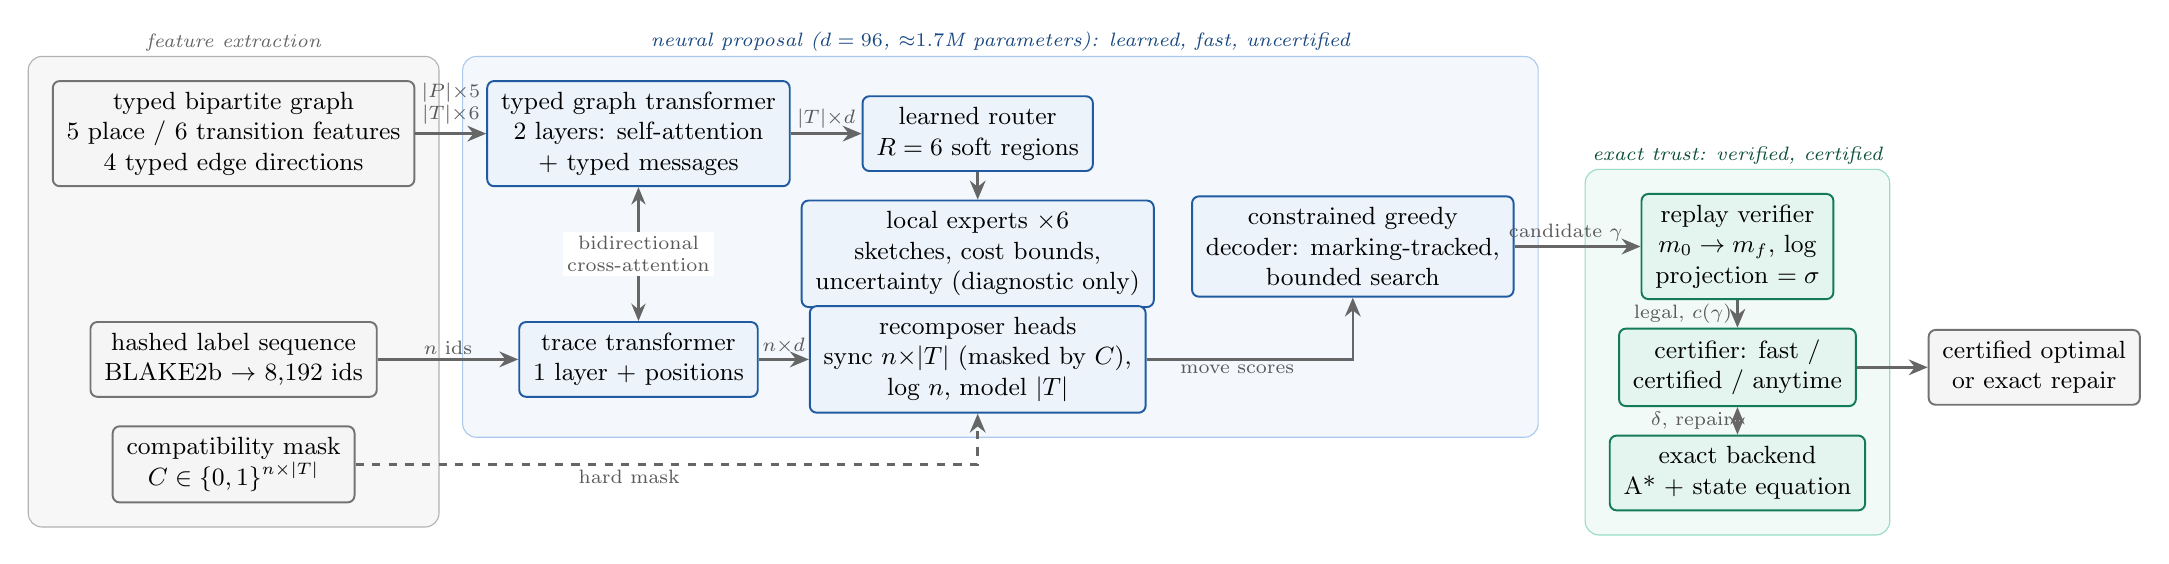
\begin{tikzpicture}[font=\small, node distance=4mm and 9mm]
% --- feature extraction ---
\node[iobox] (bip) {typed bipartite graph\\5 place / 6 transition features\\4 typed edge directions};
\node[iobox, below=17mm of bip] (hash) {hashed label sequence\\BLAKE2b $\to$ 8{,}192 ids};
\node[iobox, below=3.5mm of hash] (mask) {compatibility mask\\$C \in \{0,1\}^{n \times |T|}$};
% --- neural model ---
\node[learnedbox, right=of bip] (gt) {typed graph transformer\\2 layers: self-attention\\$+$ typed messages};
\node[learnedbox] (tt) at (gt |- hash) {trace transformer\\1 layer $+$ positions};
\node[learnedbox, right=of gt] (router) {learned router\\$R = 6$ soft regions};
\node[learnedbox, below=3.5mm of router] (exp) {local experts $\times 6$\\sketches, cost bounds,\\uncertainty (diagnostic only)};
\node[learnedbox] (rec) at (router |- tt) {recomposer heads\\sync $n {\times} |T|$ (masked by $C$),\\log $n$, model $|T|$};
\coordinate (encmid) at ($(router.east)!0.5!(rec.east)$);
\node[learnedbox, right=of encmid, anchor=west] (dec) {constrained greedy\\decoder: marking-tracked,\\bounded search};
% --- exact trust ---
\node[exactbox, right=16mm of dec] (ver) {replay verifier\\$m_0 \to m_f$, log\\projection $= \sigma$};
\node[exactbox, below=3.5mm of ver] (cert) {certifier: fast /\\certified / anytime};
\node[exactbox, below=3.5mm of cert] (exact) {exact backend\\A* $+$ state equation};
\node[iobox, right=9mm of cert] (out) {certified optimal\\or exact repair};
% --- flows ---
\draw[flow] (bip) -- node[flowlab, above=0.5mm] {$|P| {\times} 5$\\$|T| {\times} 6$} (gt);
\draw[flow] (hash) -- node[flowlab, above] {$n$ ids} (tt);
\draw[biflow] (gt) -- node[flowlab, fill=white] {bidirectional\\cross-attention} (tt);
\draw[flow] (gt) -- node[flowlab, above] {$|T| {\times} d$} (router);
\draw[flow] (tt) -- node[flowlab, above] {$n {\times} d$} (rec);
\draw[flow] (router) -- (exp);
\draw[flow, dashed] (mask.east) -| node[flowlab, below, pos=0.22] {hard mask} (rec.south);
\draw[flow] (rec.east) -| node[flowlab, below, pos=0.22] {move scores} (dec.south);
\draw[flow] (dec) -- node[flowlab, above, xshift=-1.5mm] {candidate $\gamma$} (ver);
\draw[flow] (ver) -- node[flowlab, left] {legal, $c(\gamma)$} (cert);
\draw[biflow] (cert) -- node[flowlab, left] {$\delta$, repair} (exact);
\draw[flow] (cert) -- (out);
% --- stage backgrounds ---
\begin{scope}[on background layer]
\node[stagebg, fill=black!3, draw=black!30] (featbg) [fit=(bip)(hash)(mask)] {};
\node[stagebg, fill=seriesblue!5, draw=seriesblue!40] (learnbg) [fit=(gt)(tt)(router)(exp)(rec)(dec)] {};
\node[stagebg, fill=seriesaqua!6, draw=seriesaqua!45] (trustbg) [fit=(ver)(cert)(exact)] {};
\end{scope}
\node[stagelab, text=black!60, anchor=south] at (featbg.north) {feature extraction};
\node[stagelab, text=seriesblue!60!black, anchor=south] at (learnbg.north) {neural proposal ($d = 96$, ${\approx}1.7$M parameters): learned, fast, uncertified};
\node[stagelab, text=seriesaqua!45!black, anchor=south] at (trustbg.north) {exact trust: verified, certified};
\end{tikzpicture}}
\caption{The LARA architecture: coupled net and trace encoders feed the scoring heads; a constrained greedy decoder emits a fireable candidate that is verified by replay and certified or repaired by the exact backend.}
\label{fig:architecture}
\end{figure}

\subsection{Neural Scoring: Three Questions per Net and Trace Pair}
\label{sec:architecture}

\emph{Input:} the encoded pair of Section~\ref{sec:encoding}. \emph{Output:} scored answers to the three questions any aligner faces. For every event $i$ and transition $j$: how plausible is it that event $i$ synchronizes with exactly transition $j$ (synchronous scores $\mathrm{sync} \in \mathbb{R}^{n \times |T|}$, masked by $C$)? For every event: how plausible is it that it is a deviation to be skipped (log-move scores in $\mathbb{R}^n$)? For every transition: how plausible is it that the model requires it although no event matches (model-move scores in $\mathbb{R}^{|T|}$)? Only these move scores travel further down the pipeline, to the decoder of Section~\ref{sec:decoding}. The model is deliberately small, roughly 1.7M parameters (hidden dimension $d = 96$), and runs comfortably on CPU.

\textbf{Two coupled encoders.} A graph transformer reads the net: over two rounds, every place and transition refines its representation by attending to all other nodes and exchanging messages with its neighbors, separately per arc type and direction, so structural context accumulates in each node. A sequence transformer \cite{Vaswani2017} reads the trace, embedding events through the \emph{same} label identifiers as transitions, so an event and its label-compatible transitions start from the same representation. One round of bidirectional cross-attention couples the two encoders: every event looks at the transitions that could explain it, and every transition looks at the events that could justify firing it. This coupling makes all scores \emph{trace-dependent}: the same net is scored differently depending on where the trace deviates.

\textbf{Move-scoring heads.} The synchronous score of event $i$ and transition $j$ compares their two representations (a scaled bilinear form), hard-masked by $C$; row $i$ is the model's belief about \emph{which concrete transition} event $i$ should synchronize with, and this is where duplicate-label resolution happens. Log-move and model-move scores are read off the event and transition representations directly.

\textbf{A diagnostic decomposition branch.} A learned router additionally assigns transitions and events softly to $R = 6$ latent regions, and per region a small head predicts a local deviation sketch (out of $S = 4$ patterns), lower and upper cost bounds, and an uncertainty estimate; the summed upper bounds are the model's estimate of the total alignment cost, supervised against the optimum. Figure~\ref{fig:regions} illustrates the branch. It is the learned analogue of decomposition-based conformance checking \cite{Aalst2013,Verbeek2016}: the partition is predicted per net and trace pair rather than fixed structurally. This branch is \emph{diagnostic only}: its outputs never reach the decoder or the exact search, since a learned cost bound carries no admissibility guarantee.

\begin{figure}
\begin{minipage}[t]{0.505\textwidth}
\centering
\resizebox{\linewidth}{!}{%
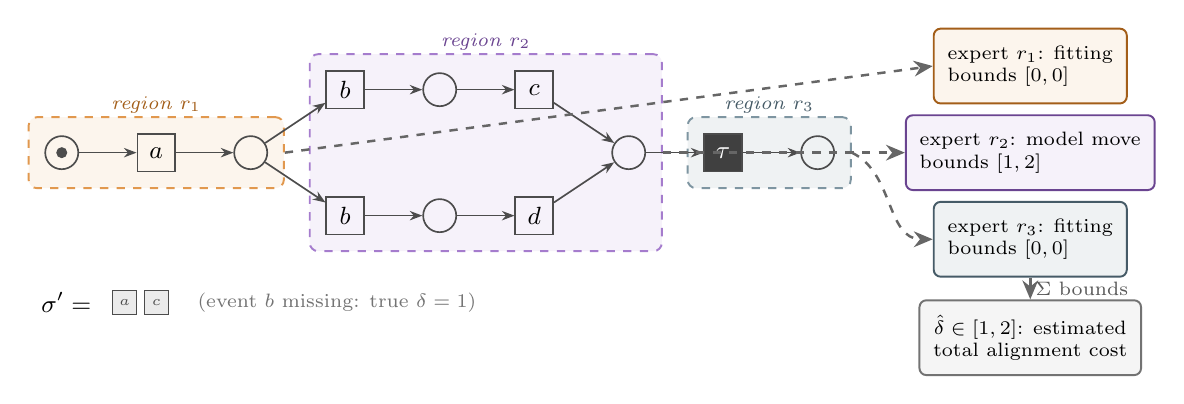
\begin{tikzpicture}[font=\small]
% the net, colored by the latent regions predicted for this trace
\node[place] (p0) at (0,0) {};
\fill[black!70] (p0.center) circle (0.7mm);
\node[trans] (ta) at (1.2,0) {$a$};
\node[place] (p1) at (2.4,0) {};
\node[trans] (t1) at (3.6,0.8) {$b$};
\node[trans] (t2) at (3.6,-0.8) {$b$};
\node[place] (p2) at (4.8,0.8) {};
\node[place] (p3) at (4.8,-0.8) {};
\node[trans] (tc) at (6.0,0.8) {$c$};
\node[trans] (td) at (6.0,-0.8) {$d$};
\node[place] (p4) at (7.2,0) {};
\node[invtrans] (tt) at (8.4,0) {$\tau$};
\node[place] (p5) at (9.6,0) {};
\draw[netarc] (p0) -- (ta); \draw[netarc] (ta) -- (p1);
\draw[netarc] (p1) -- (t1); \draw[netarc] (p1) -- (t2);
\draw[netarc] (t1) -- (p2); \draw[netarc] (t2) -- (p3);
\draw[netarc] (p2) -- (tc); \draw[netarc] (p3) -- (td);
\draw[netarc] (tc) -- (p4); \draw[netarc] (td) -- (p4);
\draw[netarc] (p4) -- (tt); \draw[netarc] (tt) -- (p5);
% the trace this partition was predicted for
\node[font=\small, anchor=east] at (0.5,-1.9) {$\sigma' = $};
\draw[black!70, fill=black!8] (0.65,-2.05) rectangle +(0.3,0.3);
\node[font=\tiny, text=black!70] at (0.8,-1.9) {$a$};
\draw[black!70, fill=black!8] (1.05,-2.05) rectangle +(0.3,0.3);
\node[font=\tiny, text=black!70] at (1.2,-1.9) {$c$};
\node[font=\scriptsize, text=black!55, anchor=west] at (1.6,-1.9)
  {(event $b$ missing: true $\delta = 1$)};
% latent region hulls
\begin{scope}[on background layer]
\node[regbox, draw=regamber!80, fill=regamber!8, fit=(p0)(ta)(p1)] (r1) {};
\node[regbox, draw=regplum!80, fill=regplum!8, fit=(t1)(t2)(p2)(p3)(tc)(td)(p4)] (r2) {};
\node[regbox, draw=regslate!80, fill=regslate!10, fit=(tt)(p5)] (r3) {};
\end{scope}
\node[reglab, text=regamber!75!black, anchor=south] at (r1.north) {region $r_1$};
\node[reglab, text=regplum!75!black, anchor=south] at (r2.north) {region $r_2$};
\node[reglab, text=regslate!75!black, anchor=south] at (r3.north) {region $r_3$};
% per-region experts
\node[larabox, draw=regamber!75!black, fill=regamber!8, font=\scriptsize, align=left] (e1) at (12.3,1.1) {expert $r_1$: fitting\\bounds $[0,0]$};
\node[larabox, draw=regplum!75!black, fill=regplum!8, font=\scriptsize, align=left] (e2) at (12.3,0) {expert $r_2$: model move\\bounds $[1,2]$};
\node[larabox, draw=regslate!75!black, fill=regslate!10, font=\scriptsize, align=left] (e3) at (12.3,-1.1) {expert $r_3$: fitting\\bounds $[0,0]$};
\node[iobox, font=\scriptsize] (sum) at (12.3,-2.35) {$\hat\delta \in [1,2]$: estimated\\total alignment cost};
\draw[flow, dashed] (r1.east) -- (e1.west);
\draw[flow, dashed] (r2.east) -- (e2.west);
\draw[flow, dashed] (r3.east) to[out=-25,in=180] (e3.west);
\draw[flow] (e3.south) -- node[flowlab, right] {$\Sigma$ bounds} (sum.north);
\end{tikzpicture}}
\caption{The diagnostic decomposition branch on a duplicate-label choice net, for a trace $\sigma'$ that skips event $b$: the router predicts latent regions (three of $R = 6$ shown), local experts predict sketches and cost bounds, and the summed bounds estimate the alignment cost; all outputs are diagnostic only.}
\label{fig:regions}
\end{minipage}\hfill
\begin{minipage}[t]{0.465\textwidth}
\centering
\resizebox{\linewidth}{!}{%
\begin{tikzpicture}[font=\small]
% the system net: a duplicate-label choice net with an invisible join
\node[place] (p0) at (0,0) {};
\fill[black!70] (p0.center) circle (0.7mm);
\node[trans] (ta) at (1.2,0) {$a$};
\node[place] (p1) at (2.4,0) {};
\node[trans] (t1) at (3.6,0.8) {$b$};
\node[trans] (t2) at (3.6,-0.8) {$b$};
\node[place] (p2) at (4.8,0.8) {};
\node[place] (p3) at (4.8,-0.8) {};
\node[trans] (tc) at (6.0,0.8) {$c$};
\node[trans] (td) at (6.0,-0.8) {$d$};
\node[place] (p4) at (7.2,0) {};
\node[invtrans] (tt) at (8.4,0) {$\tau$};
\node[place] (p5) at (9.6,0) {};
\draw[netarc] (p0) -- (ta); \draw[netarc] (ta) -- (p1);
\draw[netarc] (p1) -- (t1); \draw[netarc] (p1) -- (t2);
\draw[netarc] (t1) -- (p2); \draw[netarc] (t2) -- (p3);
\draw[netarc] (p2) -- (tc); \draw[netarc] (p3) -- (td);
\draw[netarc] (tc) -- (p4); \draw[netarc] (td) -- (p4);
\draw[netarc] (p4) -- (tt); \draw[netarc] (tt) -- (p5);
\node[font=\scriptsize, text=black!60, below=0.5mm of p0] {$m_0$};
\node[font=\scriptsize, text=black!60, below=0.5mm of p5] {$m_f$};
\node[font=\scriptsize, text=black!60, above=0.5mm of ta] {$t_a$};
\node[font=\scriptsize, text=black!60, above=0.5mm of tc] {$t_c$};
\node[font=\scriptsize, text=black!60, below=0.5mm of td] {$t_d$};
% synchronous scores for the ambiguous event b
\node[scorebadge, above=1.2mm of t1] (s1) {$t_1$: sync $0.92$};
\node[scorebadgelow, below=1.2mm of t2] (s2) {$t_2$: sync $0.08$};
% the trace
\node[font=\small, anchor=east] at (0.55,-2.36) {$\sigma =$};
\pic at (1.15,-2.36) {trcfrag};
% the decoded candidate as a two-row alignment table
\node[font=\small, anchor=east] at (3.05,-2.36) {$\gamma =$};
\node[alcell, anchor=west, fill=black!4] (L0) at (3.15,-2.1) {$a$};
\node[alcell, anchor=west, fill=black!4] (L1) at (4.45,-2.1) {$b$};
\node[alcell, anchor=west, fill=black!4] (L2) at (5.75,-2.1) {$c$};
\node[alcell, anchor=west, fill=black!4] (L3) at (7.05,-2.1) {$\gg$};
\node[alcell, anchor=west, fill=seriesblue!7] (M0) at (3.15,-2.62) {$t_a$};
\node[alcell, anchor=west, fill=seriesblue!18, draw=seriesblue!75!black] (M1) at (4.45,-2.62) {$t_1$};
\node[alcell, anchor=west, fill=seriesblue!7] (M2) at (5.75,-2.62) {$t_c$};
\node[alcell, anchor=west, fill=seriesblue!7] (M3) at (7.05,-2.62) {$\tau$};
% the decoder rule applied per move
\node[font=\scriptsize, text=black!55, anchor=south] at (3.8,-1.87) {unique match};
\node[font=\scriptsize, text=seriesblue!70!black, anchor=south] at (5.1,-1.87) {arg\,max sync};
\node[font=\scriptsize, text=black!55, anchor=south] at (6.4,-1.87) {unique match};
\node[font=\scriptsize, text=black!55, anchor=south] at (7.7,-1.87) {search to $m_f$};
% the tracked marking
\node[font=\scriptsize, text=black!55, anchor=west] at (3.15,-3.15)
  {tracked marking: $[p_0] \xrightarrow{t_a} [p_1] \xrightarrow{t_1} [p_2] \xrightarrow{t_c} [p_4] \xrightarrow{\tau} [p_5] = m_f$};
\end{tikzpicture}}
\caption{Guided decoding on the same net for the fitting trace $\sigma = \langle a, b, c \rangle$: at event $b$ two enabled transitions carry the label, so the synchronous scores, informed by the suffix, select $t_1$; the final bounded search reaches $m_f$ through the invisible transition. Every move fires on the tracked marking.}
\label{fig:decoding}
\end{minipage}
\end{figure}

\subsection{Decoding, Verification, and Certification: From Scores to a Certified Alignment}
\label{sec:decoding}

\emph{Input:} the system net, the trace $\sigma$, and the move scores of Section~\ref{sec:architecture}. \emph{Output:} a legal alignment whose guarantee depends on the chosen mode: certified optimal, exactly repaired, or a verified upper bound. Algorithm~\ref{alg:decode} shows the complete procedure and Figure~\ref{fig:decoding} traces its decoding phase on the running example. The learned scores are consumed exclusively during decoding (lines 1 to 12); the verifier and certifier judge only the resulting alignment object, so the trust boundary of Figure~\ref{fig:architecture} is crossed by an alignment, never by neural output.

\begin{algorithm}
\caption{Guided greedy decoding, verification, and certification.}
\label{alg:decode}
\footnotesize
\begin{algorithmic}[1]
\Require system net $SN = (N, m_0, m_f)$, trace $\sigma = \langle a_1, \ldots, a_n \rangle$, move scores of Section~\ref{sec:architecture}, mode
\State $\gamma \gets \langle\,\rangle$;\quad $m \gets m_0$ \Comment{every appended model component is fired on $m$}
\For{$i = 1, \ldots, n$}
  \State $E \gets \{\, t \text{ enabled at } m \mid \lambda(t) = a_i \,\}$
  \If{$|E| = 1$} append the synchronous move $(a_i, t)$ \Comment{forced by the marking}
  \ElsIf{$|E| > 1$} append $(a_i, t^\ast)$ with $t^\ast = \arg\max_{t \in E} \mathrm{sync}(i, t)$ \Comment{duplicate labels}
  \Else{} BFS over model moves from $m$, depth $\leq 8$: invisible transitions first, then by model-move score
    \If{the search reaches a marking enabling $a_i$} append its model moves, then the synchronous move
    \Else{} append the log move $(a_i, \gg)$ \Comment{the net cannot catch up}
    \EndIf
  \EndIf
\EndFor
\State append model moves reaching $m_f$ (bounded search, depth $\leq 32$)
\State \emph{verify}: replay $\gamma$ from $m_0$; check that $m_f$ is reached and the log projection equals $\sigma$; compute $c(\gamma)$
\If{mode is \textsc{fast}} \Return $\gamma$ with the verified upper bound $c(\gamma) \geq \delta(\sigma, SN)$
\Else{} compute $\delta$ by exact A*; \Return $\gamma$ certified if $c(\gamma) = \delta$, else the exact alignment as repair
\EndIf
\end{algorithmic}
\end{algorithm}

The decoder walks over the trace once, left to right, and always knows the current marking, so the candidate $\gamma$ is fireable by construction; the diagnostic regions of Section~\ref{sec:architecture} play no role here. The marking forces everything that can be forced: an event with a unique enabled match synchronizes without any learned knowledge (line 4), and an event that no short model-move sequence can enable becomes a log move (line 8). The learned scores settle exactly the two choices a greedy pass would otherwise guess. Among several enabled transitions carrying the event's label, the duplicate-label situation, the synchronous score selects the identity (line 5): a structural tie-break could only guess between look-alike duplicates, while the score is computed with a view of the entire trace and knows which branch the suffix supports. When the net must first catch up (line 6), the model-move scores decide which routing path through the net the model most plausibly took. The approach is similar to token-based replay \cite{Rozinat2008,Berti2021}, which also walks the trace once and fires transitions on a tracked marking, and to alignment approximation \cite{Schuster2021}, which also trades optimality for speed while keeping an alignment-shaped output; unlike both, every discretionary choice is settled by the learned trace-aware scores, and the result is replay-verified and, on demand, certified or repaired exactly.

Unlike exact aligners, which explore the synchronous product, may revise any decision, and provably return the cheapest alignment \cite{Zelst2018,Dongen2018}, the bounded searches of lines 6 and 12 explore model moves only, stop at the \emph{first} enabling marking rather than the cheapest one, and never revisit a commitment: they guarantee that the candidate can be replayed, not that it is cheap. This is the failure mode analyzed in Section~\ref{sec:failure} and the reason the exact layer stays in the loop: the verifier (line 13) establishes legality and the cost $c(\gamma)$ by replay, and the certifier (lines 14 and 15) delivers the requested guarantee by cost equality (Section~\ref{sec:preliminaries}) or exact repair. A third mode, \textsc{anytime}, degrades gracefully on exact-backend timeouts and returns the best available bounds. A precomputed per-net runtime keeps the searches cheap, so the neural forward pass dominates fast-mode wall time.

% Width of the toy training figure as a fraction of the text width:
% adjust this single macro to resize the whole figure.
\newcommand{\trainingfigwidth}{0.7\textwidth}
\begin{figure}[b]
\centering
\resizebox{\trainingfigwidth}{!}{%
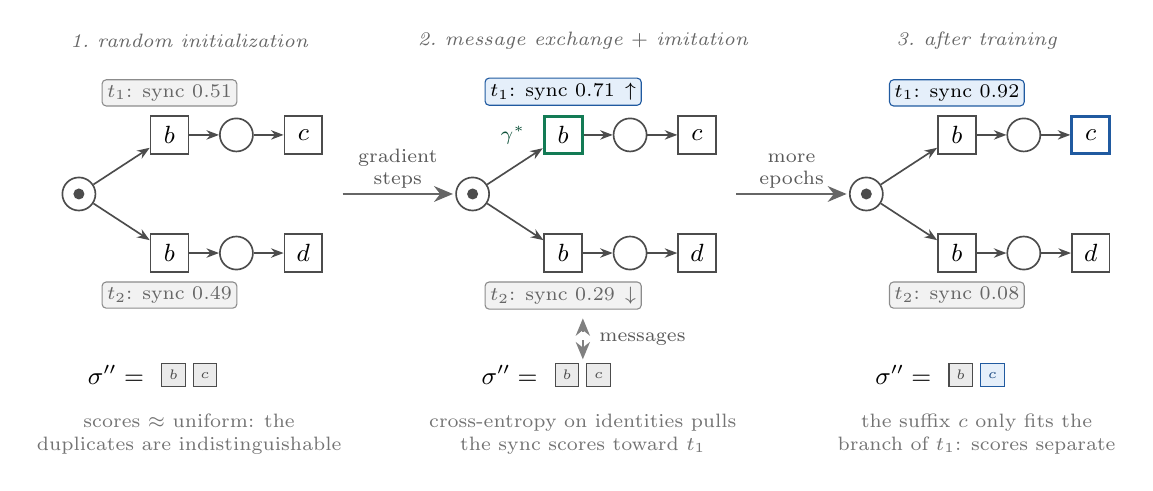
\begin{tikzpicture}[font=\small]
% panel 1: randomly initialized model
\node[stagelab, text=black!60] at (1.4,1.95) {1.\ random initialization};
\node[place] (pa) at (0,0) {};
\fill[black!70] (pa.center) circle (0.7mm);
\node[trans] (ta1) at (1.15,0.75) {$b$};
\node[trans] (ta2) at (1.15,-0.75) {$b$};
\node[place] (qa1) at (2.0,0.75) {};
\node[place] (qa2) at (2.0,-0.75) {};
\node[trans] (ca) at (2.85,0.75) {$c$};
\node[trans] (da) at (2.85,-0.75) {$d$};
\draw[netarc] (pa) -- (ta1); \draw[netarc] (pa) -- (ta2);
\draw[netarc] (ta1) -- (qa1); \draw[netarc] (ta2) -- (qa2);
\draw[netarc] (qa1) -- (ca); \draw[netarc] (qa2) -- (da);
\node[scorebadgelow, above=1.1mm of ta1] {$t_1$: sync $0.51$};
\node[scorebadgelow, below=1.1mm of ta2] {$t_2$: sync $0.49$};
\draw[black!70, fill=black!8] (1.05,-2.45) rectangle +(0.3,0.3);
\node[font=\tiny, text=black!70] at (1.2,-2.3) {$b$};
\draw[black!70, fill=black!8] (1.45,-2.45) rectangle +(0.3,0.3);
\node[font=\tiny, text=black!70] at (1.6,-2.3) {$c$};
\node[font=\small, anchor=east] at (0.95,-2.3) {$\sigma'' =$};
\node[font=\scriptsize, text=black!55, align=center] at (1.4,-3.05)
  {scores $\approx$ uniform: the\\duplicates are indistinguishable};
% panel 2: message exchange and imitation of the exact teacher
\node[stagelab, text=black!60] at (6.4,1.95) {2.\ message exchange $+$ imitation};
\node[place] (pb) at (5.0,0) {};
\fill[black!70] (pb.center) circle (0.7mm);
\node[trans, draw=seriesaqua!70!black, line width=1.1pt] (tb1) at (6.15,0.75) {$b$};
\node[trans] (tb2) at (6.15,-0.75) {$b$};
\node[place] (qb1) at (7.0,0.75) {};
\node[place] (qb2) at (7.0,-0.75) {};
\node[trans] (cb) at (7.85,0.75) {$c$};
\node[trans] (db) at (7.85,-0.75) {$d$};
\draw[netarc] (pb) -- (tb1); \draw[netarc] (pb) -- (tb2);
\draw[netarc] (tb1) -- (qb1); \draw[netarc] (tb2) -- (qb2);
\draw[netarc] (qb1) -- (cb); \draw[netarc] (qb2) -- (db);
\node[font=\scriptsize, text=seriesaqua!45!black, left=1mm of tb1] {$\gamma^\ast$};
\node[scorebadge, above=1.1mm of tb1] {$t_1$: sync $0.71\,\uparrow$};
\node[scorebadgelow, below=1.1mm of tb2] {$t_2$: sync $0.29\,\downarrow$};
\draw[black!70, fill=black!8] (6.05,-2.45) rectangle +(0.3,0.3);
\node[font=\tiny, text=black!70] at (6.2,-2.3) {$b$};
\draw[black!70, fill=black!8] (6.45,-2.45) rectangle +(0.3,0.3);
\node[font=\tiny, text=black!70] at (6.6,-2.3) {$c$};
\node[font=\small, anchor=east] at (5.95,-2.3) {$\sigma'' =$};
\draw[biflow, dashed, draw=black!50] (6.4,-2.1) -- (6.4,-1.58);
\node[flowlab, anchor=west] at (6.55,-1.84) {messages};
\node[font=\scriptsize, text=black!55, align=center] at (6.4,-3.05)
  {cross-entropy on identities pulls\\the sync scores toward $t_1$};
% panel 3: after training
\node[stagelab, text=black!60] at (11.4,1.95) {3.\ after training};
\node[place] (pc) at (10.0,0) {};
\fill[black!70] (pc.center) circle (0.7mm);
\node[trans] (tc1) at (11.15,0.75) {$b$};
\node[trans] (tc2) at (11.15,-0.75) {$b$};
\node[place] (qc1) at (12.0,0.75) {};
\node[place] (qc2) at (12.0,-0.75) {};
\node[trans, draw=seriesblue!75!black, line width=1.1pt] (cc) at (12.85,0.75) {$c$};
\node[trans] (dc) at (12.85,-0.75) {$d$};
\draw[netarc] (pc) -- (tc1); \draw[netarc] (pc) -- (tc2);
\draw[netarc] (tc1) -- (qc1); \draw[netarc] (tc2) -- (qc2);
\draw[netarc] (qc1) -- (cc); \draw[netarc] (qc2) -- (dc);
\node[scorebadge, above=1.1mm of tc1] {$t_1$: sync $0.92$};
\node[scorebadgelow, below=1.1mm of tc2] {$t_2$: sync $0.08$};
\draw[black!70, fill=black!8] (11.05,-2.45) rectangle +(0.3,0.3);
\node[font=\tiny, text=black!70] at (11.2,-2.3) {$b$};
\draw[seriesblue!75!black, fill=seriesblue!12] (11.45,-2.45) rectangle +(0.3,0.3);
\node[font=\tiny, text=seriesblue!60!black] at (11.6,-2.3) {$c$};
\node[font=\small, anchor=east] at (10.95,-2.3) {$\sigma'' =$};
\node[font=\scriptsize, text=black!55, align=center] at (11.4,-3.05)
  {the suffix $c$ only fits the\\branch of $t_1$: scores separate};
% progression arrows
\draw[flow] (3.35,0) -- node[flowlab, above] {gradient\\steps} (4.75,0);
\draw[flow] (8.35,0) -- node[flowlab, above] {more\\epochs} (9.75,0);
\end{tikzpicture}}
\caption{Toy example of how the foundation model is trained, on a duplicate-label choice whose branches continue with $c$ and $d$, for the trace $\sigma'' = \langle b, c \rangle$: the randomly initialized model scores both transitions labeled $b$ alike; during training, net and trace representations exchange messages while the cross-entropy on transition identities pulls the synchronous scores toward the transition fired by the exact teacher alignment $\gamma^\ast$; after convergence the checkpoint recognizes that the suffix $c$ only fits the branch of $t_1$, yielding scores like those of Figure~\ref{fig:decoding}.}
\label{fig:training}
\end{figure}

\subsection{Exact-Labeled Training Data}
\label{sec:data}

The scoring heads are trained by imitation on synthetic event logs paired with synthetic Petri-net representations. Each generated trace-model pair is labeled by the exact backend, so every training target is a provably optimal alignment \emph{with transition identities}. The generator controls how often duplicate labels, invisible routing, concurrency, non-free-choice structure, and overlapping deviations appear, while the exact aligner supplies the supervision used by the move heads. Activity names are deliberately unimportant: with the hashed labels of Section~\ref{sec:encoding}, the model learns structural and behavioral relations rather than a fixed vocabulary.

Each example is produced at the level of a \emph{behavior family}, not as an isolated trace. The generator balances four motifs that expose the ambiguities of alignment: ordinary block trees and isomorphic renamings, duplicate-prefix activities and equivalent silent routing, true parallelism and explicit interleaving, and canonical blocks versus M-pattern non-free-choice nets. For each family, two Petri-net representations and two observed traces are created; corruption is applied once at the visible-label level, mixing clean behavior with deletion, insertion, substitution, repetition, swaps, and prefix or suffix truncation, so equivalent representations see the same noisy trace. The exact backend then aligns every representation-trace pair, replay-verifies the alignment, and rejects families whose equivalent variants disagree in optimal cost. Splits are assigned before representation expansion, preventing behavior leakage. The reference corpus contains 2{,}048 training examples plus 512 validation and 512 test examples, balanced across the four motifs, with test traces averaging 3.6 events and optimal costs 0 to 7.

\subsection{Training Objective and Procedure}
\label{sec:training}

The exact aligner already answers every alignment question, only too slowly, so the model learns to \emph{imitate} it on the corpus of Section~\ref{sec:data}, well enough that the greedy decoder of Section~\ref{sec:decoding} makes the same choices at a fraction of the cost; Figure~\ref{fig:training} illustrates this imitation on a toy duplicate-label pair. Every term of the loss holds one output of Section~\ref{sec:architecture} against what the exact aligner did:
\begin{equation*}
\mathcal{L} = w_m (\mathcal{L}_{\mathrm{sync}} + \mathcal{L}_{\mathrm{log}} + \mathcal{L}_{\mathrm{model}}) + w_c \mathcal{L}_{\mathrm{cost}} + w_b \mathcal{L}_{\mathrm{bound}} + w_\ell \mathcal{L}_{\mathrm{bal}} + w_e \mathcal{L}_{\mathrm{ent}}.
\end{equation*}
The first three terms make the model imitate the moves of the optimal alignment and correspond to the three alignment questions of Section~\ref{sec:architecture}. $\mathcal{L}_{\mathrm{sync}}$ asks whether the model points to the transition the optimal alignment actually fired: a cross-entropy over transition \emph{identities} rather than labels, which is precisely what teaches duplicate-label resolution. $\mathcal{L}_{\mathrm{log}}$ asks whether the model recognizes the events the optimum skipped, and $\mathcal{L}_{\mathrm{model}}$ whether it recognizes the transitions the optimum fired without a matching event; both are binary cross-entropies. The remaining terms train the diagnostic decomposition branch. $\mathcal{L}_{\mathrm{cost}}$ compares the summed regional upper bounds with the optimal cost $\delta$ (smooth L1), so the regions together must account for the total deviation of the trace. The last three terms shape the regions themselves: $\mathcal{L}_{\mathrm{bound}}$ penalizes assignments in which two transitions connected to the same place fall into different regions, so that regions are connected fragments of the net; $\mathcal{L}_{\mathrm{bal}}$ penalizes variance in region sizes, so that no single region absorbs the whole net; and $\mathcal{L}_{\mathrm{ent}}$ penalizes the entropy of the soft assignments, so that every node is placed decisively. The weights ($w_m = 1.0$, $w_c = 0.03$, $w_b = w_\ell = 0.01$, $w_e = 0.001$) keep imitation dominant: the decomposition is a regularized diagnostic, not the primary objective.


The procedure itself is standard and computationally modest, which matters for a foundation model that is trained once and then reused: with AdamW, label remapping during training, and early stopping settings recorded in the repository (Section~\ref{sec:implementation}), the reference run uses 50 epochs of roughly 41 seconds each on a single CPU, reaching its best validation loss at epoch 49 (Figure~\ref{fig:panels}, left). Validation loss is lower than training loss because the training pass uses dropout and random label remapping, while validation keeps labels fixed; deciding which events are deviations remains the hardest sub-task.

\begin{figure}
\centering
\begin{minipage}[t]{0.48\linewidth}
\centering
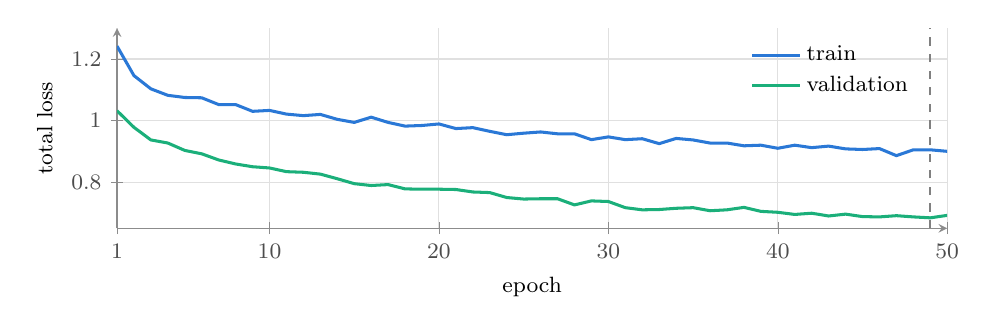
\begin{tikzpicture}
\begin{axis}[
  larapanel,
  xlabel={epoch},
  ylabel={total loss},
  xmin=1, xmax=50,
  ymin=0.65, ymax=1.30,
  xtick={1,10,20,30,40,50},
  legend pos=north east,
]
\addplot[seriesblue] coordinates {(1,1.242)(2,1.146)(3,1.103)(4,1.082)(5,1.075)(6,1.074)(7,1.052)(8,1.052)(9,1.030)(10,1.033)(11,1.021)(12,1.016)(13,1.020)(14,1.004)(15,0.994)(16,1.011)(17,0.994)(18,0.982)(19,0.984)(20,0.989)(21,0.974)(22,0.977)(23,0.965)(24,0.954)(25,0.959)(26,0.963)(27,0.957)(28,0.957)(29,0.938)(30,0.947)(31,0.938)(32,0.941)(33,0.925)(34,0.942)(35,0.937)(36,0.927)(37,0.927)(38,0.918)(39,0.920)(40,0.910)(41,0.920)(42,0.912)(43,0.917)(44,0.908)(45,0.906)(46,0.909)(47,0.886)(48,0.905)(49,0.905)(50,0.900)};
\addlegendentry{train}
\addplot[seriesaqua] coordinates {(1,1.032)(2,0.978)(3,0.937)(4,0.927)(5,0.903)(6,0.892)(7,0.872)(8,0.859)(9,0.850)(10,0.846)(11,0.834)(12,0.832)(13,0.826)(14,0.811)(15,0.795)(16,0.789)(17,0.792)(18,0.778)(19,0.777)(20,0.777)(21,0.776)(22,0.768)(23,0.766)(24,0.750)(25,0.745)(26,0.746)(27,0.746)(28,0.726)(29,0.739)(30,0.737)(31,0.717)(32,0.710)(33,0.711)(34,0.715)(35,0.717)(36,0.707)(37,0.710)(38,0.718)(39,0.705)(40,0.702)(41,0.695)(42,0.699)(43,0.690)(44,0.696)(45,0.688)(46,0.687)(47,0.691)(48,0.687)(49,0.684)(50,0.692)};
\addlegendentry{validation}
\addplot[black!50, dashed, line width=0.7pt] coordinates {(49,0.65)(49,1.30)};
\end{axis}
\end{tikzpicture}
\end{minipage}\hfill
\begin{minipage}[t]{0.48\linewidth}
\centering
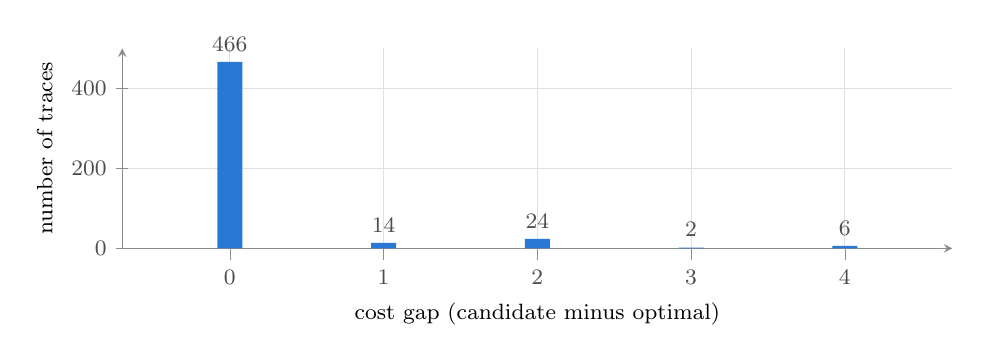
\begin{tikzpicture}
\begin{axis}[
  larapanel,
  ybar,
  bar width=9pt,
  xlabel={cost gap (candidate minus optimal)},
  ylabel={number of traces},
  xmin=-0.7, xmax=4.7,
  ymin=0, ymax=500,
  xtick={0,1,2,3,4},
  nodes near coords,
  every node near coord/.append style={font=\footnotesize, color=black!70},
]
\addplot[fill=seriesblue, draw=none] coordinates {(0,466)(1,14)(2,24)(3,2)(4,6)};
\end{axis}
\end{tikzpicture}
\end{minipage}
\caption{Left: total loss per epoch of the reference run (dashed line: best validation epoch 49). Right: cost-gap distribution on the test split ($n = 512$); the tail is short, with no gap above four.}
\label{fig:panels}
\end{figure}

\section{Implementation and Assessment}
\label{sec:assessment}

\subsection{Implementation and Reproducibility}
\label{sec:implementation}

LARA is implemented in Python on top of PyTorch and PM4Py \cite{Berti2023} and is available as open source at \url{https://github.com/fit-alessandro-berti/lara-align}. The repository contains the evaluated checkpoint, all result artifacts, and the scripts behind every number in this section, including the \texttt{--no-guidance} switch used in Section~\ref{sec:ablation}. For use on own data, \texttt{scripts/align\_log.py} aligns an XES log against a PNML net in any of the three modes, and a Python API accepts PM4Py objects and returns the alignment with cost, bounds, and certification status.

\textbf{Protocol.} All experiments run on a single CPU. The learned method is always evaluated in \emph{fast} mode (verified neural candidate only), so no exact repair contaminates learned metrics; the exact optimum of the PM4Py state-equation A* aligner serves as ground truth for every sample. The metrics instantiate the research questions: the replayable (legal) rate (RQ1), the optimal-cost rate and the cost-gap distribution $c(\gamma) - \delta$ (RQ2), transition-sequence and label-level match rates (RQ3), per-family, scaling, and real-life breakdowns (RQ4), the certified-optimal rate (RQ5), and the guidance ablation (RQ6).

\subsection{In-Distribution Results}
\label{sec:indist}

Table~\ref{tab:headline} reports the held-out test split (512 examples from 128 behavior families never seen in training). Every candidate was legal: bounded-search decoding plus replay verification eliminated illegal outputs (RQ1). In 91.0\% of cases the candidate attains the exact optimum and is certified without repair by cost equality (RQ2, RQ5); the remaining 9.0\% require exact repair in certified mode.

\begin{table}
\centering
\begin{minipage}[t]{0.27\textwidth}
\vspace{0pt}
\centering
\caption{Headline results on the held-out test split ($n = 512$).}
\label{tab:headline}
\scriptsize
\setlength{\tabcolsep}{2pt}
\begin{tabular}{@{}lr@{}}
\toprule
metric & value \\
\midrule
replayable & \textbf{100.0\%} \\
optimum cost / cert. & \textbf{91.0\%} \\
transition-seq. match & 61.1\% \\
label-level match & 62.5\% \\
mean / median cost gap & 0.18 / 0.00 \\
p90 / p95 / max cost gap & 0.0 / 2.0 / 4.0 \\
\bottomrule
\end{tabular}
\end{minipage}\hfill
\begin{minipage}[t]{0.39\textwidth}
\vspace{0pt}
\centering
\caption{Guidance ablation on the test split ($n = 512$).}
\label{tab:ablation}
\scriptsize
\setlength{\tabcolsep}{2pt}
\begin{tabular}{@{}lrrr@{}}
\toprule
metric & unguid. & guided & $\Delta$ \\
\midrule
replayable & 100.0\% & 100.0\% & 0.0 \\
optimum cost & 86.9\% & \textbf{91.0\%} & +4.1 \\
transition-seq. match & 57.8\% & \textbf{61.1\%} & +3.3 \\
label-level match & 58.8\% & \textbf{62.5\%} & +3.7 \\
mean cost gap & 0.26 & \textbf{0.18} & $-$0.08 \\
dup.-prefix opt. & 68.8\% & \textbf{95.3\%} & \textbf{+26.6} \\
dup. transition & 59.4\% & \textbf{79.7\%} & \textbf{+20.3} \\
\bottomrule
\end{tabular}
\end{minipage}\hfill
\begin{minipage}[t]{0.30\textwidth}
\vspace{0pt}
\centering
\caption{The learned cost estimate against the exact optimum $\delta$ on the held-out test split ($n = 512$).}
\label{tab:costest}
\scriptsize
\setlength{\tabcolsep}{2pt}
\begin{tabular}{@{}lr@{}}
\toprule
metric & value \\
\midrule
MAE upper vs.\ $\delta$ & 0.51 \\
mean signed error & $-$0.15 \\
Pearson $r$ with $\delta$ & \textbf{0.82} \\
mean est. ($\delta = 0$) & 0.27 \\
mean est. ($\delta > 0$) & 1.78 \\
deviation detect. & \textbf{89.8\%} \\
mean interval width & 1.16 \\
interval coverage & 29.1\% \\
\bottomrule
\end{tabular}
\end{minipage}
\end{table}

The cost-gap distribution (Figure~\ref{fig:panels}, right) is sharply concentrated at zero: 466 of 512 candidates are optimal, 95\% are at most two cost units above optimum, and no gap exceeds four. Because the behavior-family corpus mixes several motifs, it produces both odd and even gaps: failures combine visible model moves, log moves, and routing detours rather than only paired model/log fast-forward errors (Section~\ref{sec:failure}).

\subsection{Guidance Ablation: What Does Learning Contribute?}
\label{sec:ablation}

Does the learned component matter, or does constrained search do all the work (RQ6)? We re-ran the evaluation on identical inputs with neural guidance disabled: the unguided decoder executes Algorithm~\ref{alg:decode} unchanged, except that its two score-driven choices become fixed structural tie-breaks. Among several enabled transitions carrying the event's label (line 5), it fires the first in a deterministic order on transition names; in the catch-up search (line 6), invisible transitions still come first, but the candidates within each group follow the same name order. Every unguided choice thus depends only on the structure of the net, never on the trace being aligned.

Table~\ref{tab:ablation} shows a targeted contribution. The constrained decoder alone is already strong, but guidance improves overall optimality by 4.1 points and its largest effect sits exactly where Figure~\ref{fig:decoding} predicts: duplicate-label transition identity. On duplicate-prefix representations, guided decoding recovers 26.6 optimality points over deterministic structural tie-breaking; structural order cannot know which branch the trace suffix implies, while the synchronous head can (RQ3, RQ6).
\subsection{Quality of the Learned Cost Estimate}
\label{sec:costest}

The diagnostic branch of Section~\ref{sec:architecture} is trained but, unlike the moves, never verified at alignment time, so its usefulness must be established empirically; Table~\ref{tab:costest} compares its output with the exact optimum on the same held-out split. As a point estimate, the summed upper bounds track the optimal cost and separate fitting from deviating traces: thresholding the estimate at 0.5 decides whether a trace deviates at all with 89.8\% accuracy, so traces can be ranked by expected deviation before any alignment is computed. As an \emph{interval}, however, the branch is still miscalibrated, predicting ranges that contain the optimum in only 29.1\% of cases; this confirms the design decision of Section~\ref{sec:architecture} that learned bounds inform the analyst and never enter the search.

\subsection{Scaling Benchmark: The Speed and Quality Threshold}
\label{sec:scaling}

To locate the regime where learned decoding pays off, a scaling benchmark generates random block-structured stress nets (nested sequence, choice, parallel, and loop blocks with duplicate labels and invisible routing transitions) of increasing size, injects deviations at rates 0.15 and 0.35, and times both methods per trace (10 samples per configuration, 30-second exact timeout). This random stress generator is separate from the balanced behavior-family training corpus.

\begin{table}
\begin{minipage}[t]{0.58\textwidth}
\centering
\caption{Scaling benchmark on random block-structured nets (10 samples per configuration; exact timeout 30 s, timeouts counted at the timeout).}
\label{tab:scaling}
\footnotesize
\setlength{\tabcolsep}{3pt}
\begin{tabular}{rrrrrrrrrr}
\toprule
size & dev.\ & $|T|$ & legal & optimal & mean gap & fast med. & exact med. & speedup & t/o \\
\midrule
 5 & 0.15 &  7 & 100\% & 90\% &  0.2 &  5.5 ms &  1.3 ms & 0.23$\times$ & 0 \\
 5 & 0.35 &  6 & 100\% & 60\% &  1.6 &  4.6 ms &  1.3 ms & 0.29$\times$ & 0 \\
10 & 0.15 & 13 & 100\% & 80\% &  1.2 &  5.0 ms &  1.8 ms & 0.36$\times$ & 0 \\
10 & 0.35 & 13 & 100\% & 50\% &  1.7 &  5.3 ms &  2.8 ms & 0.53$\times$ & 0 \\
20 & 0.15 & 28 & 100\% & 60\% &  3.6 &  6.9 ms &  2.9 ms & 0.42$\times$ & 0 \\
20 & 0.35 & 26 & 100\% & 60\% &  3.1 &  6.0 ms & 11.7 ms & \textbf{1.94$\times$} & 0 \\
40 & 0.15 & 55 & 100\% & 30\% &  8.1 &  8.7 ms & 63.9 ms & \textbf{7.34$\times$} & 0 \\
40 & 0.35 & 54 & 100\% & 44\% & 11.7 &  8.6 ms & 24.7 ms & \textbf{2.87$\times$} & 1 \\
\bottomrule
\end{tabular}
\end{minipage}\hfill
\begin{minipage}[t]{0.38\textwidth}
\vspace{0pt}
\centering
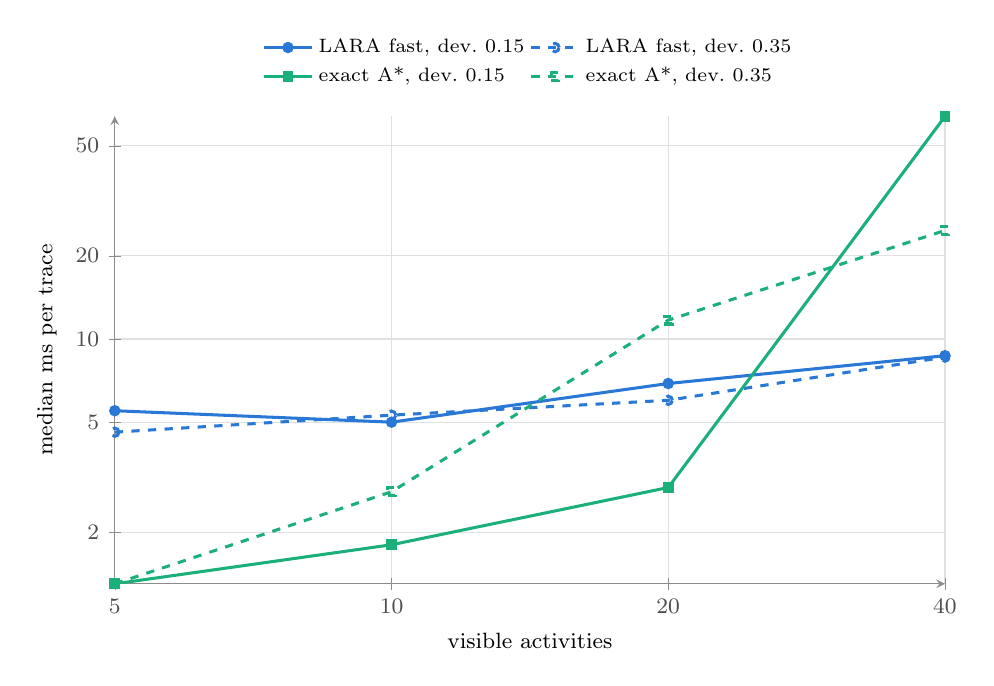
\begin{tikzpicture}
\begin{axis}[
  larachart,
  width=\linewidth,
  height=0.62\linewidth,
  xlabel={visible activities},
  ylabel={median ms per trace},
  xmode=log, log ticks with fixed point,
  xtick={5,10,20,40},
  ymode=log, log ticks with fixed point,
  ytick={1,2,5,10,20,50},
  legend style={at={(0.5,1.04)}, anchor=south, legend columns=2, font=\scriptsize},
]
\addplot[seriesblue, mark=*, mark size=1.5pt] coordinates {(5,5.5)(10,5.0)(20,6.9)(40,8.7)};
\addlegendentry{LARA fast, dev.\ 0.15}
\addplot[seriesblue, dashed, mark=o, mark size=1.5pt] coordinates {(5,4.6)(10,5.3)(20,6.0)(40,8.6)};
\addlegendentry{LARA fast, dev.\ 0.35}
\addplot[seriesaqua, mark=square*, mark size=1.4pt] coordinates {(5,1.3)(10,1.8)(20,2.9)(40,63.9)};
\addlegendentry{exact A*, dev.\ 0.15}
\addplot[seriesaqua, dashed, mark=square, mark size=1.4pt] coordinates {(5,1.3)(10,2.8)(20,11.7)(40,24.7)};
\addlegendentry{exact A*, dev.\ 0.35}
\end{axis}
\end{tikzpicture}
\captionof{figure}{Median alignment time per trace versus net size on block-structured nets (log-log). LARA stays at the forward-pass floor; exact A* degrades super-linearly, with first timeouts at size 40.}
\label{fig:scaling}
\end{minipage}
\end{table}

Three findings emerge from Table~\ref{tab:scaling} and Figure~\ref{fig:scaling}. First, LARA scales gently: the median stays between 4.6 and 8.7 ms across the ladder (the forward-pass floor plus a mild search term), while exact A* degrades super-linearly; the crossover appears at size 40 for deviation rate 0.15 and already at size 20 for deviation rate 0.35, with the first 30-second timeout at size 40. Second, legality is scale-invariant: 100\% replayable candidates at every size. Third, quality at scale remains the main limitation: the optimal-cost rate falls to 30--44\% at 40 activities. An unguided rerun shows why the learned component must justify its forward pass carefully: on this stress benchmark guidance adds little quality, while the unguided decoder runs at 0.2 to 1.2 ms per trace and overtakes exact search at every tested size.
\subsection{Zero-Shot Validation on Real-Life Logs}
\label{sec:reallife}

To test external validity, the same checkpoint was evaluated without any fine-tuning on two real-life logs: the receipt phase of a Dutch municipality's building-permit process \cite{ReceiptLog} (1{,}434 traces, 116 variants, 27 activity labels) and a road traffic fine management sample \cite{RoadTrafficLog} (100 traces, 10 variants, 10 labels). For each log a Petri net is discovered with the inductive miner \cite{Leemans2013} at noise thresholds 0.0 (perfectly fitting, so every optimal cost is 0) and 0.5 (filtered, so rarer variants genuinely deviate). The test is strictly zero-shot: the labels were never seen in training and embed only via the hash, and inductive-miner nets are dominated by invisible routing transitions (47 invisible versus 27 visible for the fitting receipt model), far from the training distribution.

Table~\ref{tab:reallife} supports four observations. \emph{Legality transfers perfectly}: 100\% replayable alignments in every configuration, so RQ1 holds across three distributions. \emph{Optimality is strong on frequent behavior, weaker in the tail}: trace-weighted optimal rates (74.6 to 100\%) sit well above variant-level rates because misses concentrate in rare, long variants; on the fitting receipt net, 82.6\% trace-weighted optimality means most real behavior is replayed without any deviation, and every miss remains a bounded upper estimate. \emph{The speed picture matches the synthetic threshold}: exact A* wins on the small road-traffic nets, but on the receipt models LARA fast overtakes exact search on a real log (16.0 versus 31.0 ms at noise 0.0, and 6.7 versus 12.7 ms at noise 0.5), and invisible-heavy discovered models are exactly where the synchronous product blows up. \emph{Guided and unguided quality are identical here}, as the ablation predicts: inductive-miner nets contain no duplicate labels, the one sub-problem where the current checkpoint's guidance pays off.

\begin{table}
\caption{Zero-shot results on real-life logs with inductive-miner models (per variant; trace-wtd.\ weights variants by frequency).}
\label{tab:reallife}
\footnotesize
\begin{tabular}{llrrrrrr}
\toprule
log & noise & net ($|P|$ / $|T_v|{+}|T_\tau|$) & legal & \multicolumn{2}{c}{optimal} & gap & \multicolumn{1}{c}{median time} \\
 & & & & variant & trace-wtd. & mean/max & LARA / exact \\
\midrule
road traffic & 0.0 & 15 / 10+10 & 100\% & 100.0\% & 100.0\% & 0 / 0 & 5.4 / 1.9 ms \\
road traffic & 0.5 & 13 / 10+7  & 100\% &  70.0\% &  94.0\% & 0.50 / 3 & 5.2 / 1.6 ms \\
receipt      & 0.0 & 45 / 27+47 & 100\% &  50.0\% &  82.6\% & 0.76 / 5 & \textbf{16.0 / 31.0 ms} \\
receipt      & 0.5 & 25 / 24+19 & 100\% &  55.2\% &  74.6\% & 0.82 / 7 & \textbf{6.7 / 12.7 ms} \\
\bottomrule
\end{tabular}
\end{table}

\subsection{Qualitative Failure Analysis}
\label{sec:failure}

The largest-gap test cases share one pattern. In a representative worst case (gap 4), the trace $\langle A, D, B, C, C, D \rangle$ comes from the concurrent-versus-interleaved family. The optimum pays two log moves, skipping the early $D$ and the duplicated $C$, while synchronizing the intended $A,B,C,D$ path. LARA instead fires $B$ and $C$ as model moves to reach a marking where the early $D$ can synchronize, then emits the later $B,C,C,D$ as log moves. The root cause is decoding-time myopia, not representation failure: greedy commitments are irrevocable, and the bounded search cannot see that skipped events reappear later, the limitation anticipated in Section~\ref{sec:decoding}.

\textbf{Summary against the research questions.} Candidates are always legal across all three tested distributions (RQ1); 91.0\% attain the exact optimum, with mean gap 0.18, p95 gap 2, and max gap 4 (RQ2); duplicate-label identity resolution is the clearest learned contribution, improving duplicate-prefix optimality from 68.8\% unguided to 95.3\% guided (RQ3, RQ6); legality generalizes everywhere, while optimality generalizes to real frequent behavior but not yet to large stress nets (RQ4); and 91.0\% of fast candidates are certified without repair by cost equality (RQ5).

\section{Discussion}
\label{sec:discussion}

\textbf{Implications.} The results support the central design decision: trust and tractability need not be traded off if the learned and exact components are given the right roles. The learned component is responsible only for speed and for guidance where structural reasoning is blind. Everything the user relies on, legality, costs, and optimality certificates, comes from replay and exact search. As a consequence, legality holds regardless of distribution shift, and lower quality appears as certified-or-repaired results rather than as silent errors. The guidance ablation carries a lesson beyond this system: constrained search alone is a strong baseline, so any learned aligner should demonstrate what learning adds.

\textbf{Limitations.} The current checkpoint is trained on balanced behavior families, but the scaling benchmark still shows a quality-at-size gap: at 40 activities, only 30--44\% of the candidates remain optimal. Training directly on larger stress-net families is the natural next step, and the unguided decoder provides the baseline that a new checkpoint must clearly exceed. A second limitation is the greedy decoder itself: its irrevocable commitments produce the detours of Section~\ref{sec:failure}, and neural-guided beam or A* search over the same learned scores would attack these detours at their root. Finally, the assessment does not yet cover larger log collections, GPU batching, or further approximate aligners \cite{Schuster2021,Padro2022,Reissner2020}, and data-aware, declarative, and object-centric settings \cite{DeLeoni2013,Aalst2020ocpn} remain open.

\textbf{Threats to validity.} Internal validity is protected by the protocol: guided and unguided runs share generator seeds and inputs, and all quality metrics are computed against exact optima. The scaling benchmark uses only 10 samples per configuration, so individual cells carry sampling noise and only the overall trend should be read. External validity rests on two real-life logs, which cannot establish generality, but the zero-shot protocol makes each transfer test strict. Construct validity rests on cost equality as the certification rule (Section~\ref{sec:preliminaries}).

\section{Conclusion}
\label{sec:conclusion}

This paper introduced LARA, an approach to Petri net trace alignment in which learning proposes and exact reasoning certifies, so the result is never less trustworthy than classical conformance checking. The name spells out the design: alignments are \emph{Learned}, by a small vocabulary-free foundation model that scores alignment moves for any net and any log without per-log training; \emph{Adaptive}, because the scores and the latent decomposition are computed anew for every net and trace pair rather than fixed structurally, and the certifier adapts its guarantee (fast, certified, anytime) to the available time; and \emph{Recombined}, because per-region sketches and cost bounds are reassembled into a global estimate, in the decomposition-and-recomposition tradition of conformance checking. Empirically, the prototype produces legal alignments for every trace across three distributions, including zero-shot transfer to real-life logs; it attains and certifies the exact optimum for 91.0\% of in-distribution traces; its learned component measurably improves duplicate-label identity resolution (95.3\% versus 68.8\% optimality on duplicate-prefix representations); and its fast path overtakes exact search on larger stress nets and on real discovered models dominated by invisible transitions.

\section*{Acknowledgements}

Funded by the European Union. This work has received funding from the European High Performance Computing Joint Undertaking (JU) and from the German Federal Ministry of Research, Technology and Space (BMFTR), the Ministry of Culture and Science of North Rhine-Westphalia (MKW NRW), and the Hessian Ministry of Science and Research, Arts and Culture (HMWK) under grant agreement No 101250682.

\bibliographystyle{ACM-Reference-Format}
\bibliography{references}

\end{document}
